
% --- Introduction à l'ECDSA ---
\begin{frame}{Introduction à l'ECDSA}
\frametitle{Elliptic Curve Digital Signature Algorithm}

\begin{itemize}
    \item L'ECDSA est un \textbf{schéma de signature numérique} basé sur la Cryptographie à Courbe Elliptique (CCE).
    \item C'est un standard essentiel pour l'authentification et l'intégrité des données (e.g., cryptomonnaies, protocoles TLS/SSL).
    \item Sa sécurité repose sur la difficulté du \textbf{Problème du Logarithme Discret sur Courbe Elliptique (ECDLP)}.
\end{itemize}

\begin{block}{Avantage Majeur : Efficacité}
    Pour un niveau de sécurité équivalent, l'ECDSA utilise des clés \textbf{beaucoup plus courtes}.
    \begin{itemize}
        \item Ex: Clé ECDSA de 256 bits $\approx$ Clé RSA de 3072 bits.
    \end{itemize}
    $\rightarrow$ Signatures réduites, calculs rapides, moindre consommation de ressources.
\end{block}
\end{frame}

% ecdlp
\begin{frame}{L'Asymétrie de l'ECDLP : L'Essence de la Sécurité}
\frametitle{Le Problème du Logarithme Discret sur Courbe Elliptique}

\begin{itemize}
    \item L'ECDLP repose sur une \textbf{fonction à sens unique} créée par l'opération de multiplication scalaire sur la courbe.
    \item Cette asymétrie garantit que la \textbf{clé privée} (l'entier $k$) reste secrète, même si la clé publique ($P$) est connue de tous.
\end{itemize}

\begin{columns}
    \column{0.5\textwidth}
    \begin{block}{Le Sens Facile (Multiplication)}
        \textbf{Objectif :} Calculer le point $P$.
        \begin{itemize}
            \item \textbf{Entrée :} Clé Privée $k$ (entier) et Point de Base $G$.
            \item \textbf{Opération :} $P = k \times G$
            \item \textbf{Résultat :} Clé Publique $P$ (point).
        \end{itemize}
        $\rightarrow$ Très rapide, facile à exécuter (quelques millisecondes).
    \end{block}
    
    \column{0.5\textwidth}
    \begin{block}{Le Sens Difficile (Logarithme)}
        \textbf{Objectif :} Trouver la clé privée $k$.
        \begin{itemize}
            \item \textbf{Entrée :} Clé Publique $P$ et Point de Base $G$.
            \item \textbf{Opération :} Trouver $k$ tel que $P = kG$.
            \item \textbf{Résultat :} Clé Privée $k$.
        \end{itemize}
        $\rightarrow$ Extrêmement lent, impossible à exécuter en temps utile (nécessite un temps exponentiel).
    \end{block}
\end{columns}

\end{frame}

% --- Opérations ECDSA ---
\begin{frame}{Les Trois Opérations Clés}
\frametitle{Protocole à Clé Publique}

L'ECDSA est structuré autour de trois opérations principales:

\begin{enumerate}
    \item \textbf{Génération des clés :}
    \begin{itemize}
        \item Une courbe elliptique et un point générateur $G$ sont choisis.
        \item Une \textbf{clé privée} secrète $d$ est sélectionnée.
        \item La \textbf{clé publique} $Q$ est calculée par $Q = d \cdot G$ (multiplication scalaire).
    \end{itemize}
    \item \textbf{Signature :}
    \begin{itemize}
        \item La clé privée $d$ est utilisée pour générer une signature unique $(r, s)$ pour le message.
    \end{itemize}
    \item \textbf{Vérification :}
    \begin{itemize}
        \item La clé publique $Q$ est utilisée pour vérifier l'authenticité de la signature $(r, s)$ et l'intégrité du message.
    \end{itemize}
\end{enumerate}
\end{frame}

% Génération des clés
\begin{frame}{Génération des Clés en Cryptographie sur Courbes Elliptiques (CCE)}
\frametitle{Du Domaine Public à la Clé Secrète}



\begin{block}{Génération de la Paire de Clés (Privée/Publique)}
    Chaque utilisateur génère sa propre paire de clés à partir des paramètres de domaine.
    \begin{itemize}
        \item \textbf{Clé Privée $k$ (Le Secret) :} Un \textbf{entier aléatoire} de grande taille, choisi dans l'intervalle $[1, n-1]$, avec $n$ l'ordre du point générateur $G$. C'est un immense nombre premier.
        \item \textbf{Clé Publique $P$ (Le Partage) :} Le point $P$ résultant de la multiplication scalaire :
        $$P = k \times G$$
    \end{itemize}
    $\rightarrow$ La clé publique $P$ est calculée à partir de $k$, mais \textbf{l'inverse est impossible} à cause de l'ECDLP.
\end{block}

\end{frame}

% signature 1
\begin{frame}{Procédure de Signature Numérique (ECDSA)}
\frametitle{Algorithme de signature}

\begin{block}{Contexte et Paramètres}
    \begin{itemize}
        \item \textbf{Paramètres Publics (connus) :} Courbe $E$, Point générateur $G$, Ordre $n$.
        \item \textbf{Clé Privée du Signataire :} $k_{priv}$ (entier secret, $1 < k_{priv} < n$).
        \item \textbf{Message :} $M$ à signer.
    \end{itemize}
\end{block}

\vspace{0.2cm}

\begin{enumerate}
    \item \textbf{Hachage du Message}
    \begin{itemize}
        \item Calculer $h = HASH(M)$, où $h$ est interprété comme un entier.
    \end{itemize}
    
    \item \textbf{Génération du Nonce Aléatoire}
    \begin{itemize}
        \item Choisir un entier aléatoire et secret $r$ (le nonce), avec $1 < r < n$.
    \end{itemize}
    
    \item \textbf{Calcul du Premier Composant ($R$)}
    \begin{itemize}
        \item Calculer le point éphémère $R = r \times G$.
        \item Extraire sa coordonnée $x_R$ et calculer $R_{sig} = x_R \pmod n$.
        \item \textbf{Note :} Si $R_{sig} = 0$, reprendre l'étape 2.
    \end{itemize}
    
    \item \textbf{Calcul du Second Composant ($S$)}
    \begin{itemize}
        \item Calculer $S = r^{-1} \times (h + R_{sig} \times k_{priv}) \pmod n$.
        \item \textbf{Note :} $r^{-1}$ est l'inverse modulaire de $r$ modulo $n$. Si $S = 0$, reprendre l'étape 2.
    \end{itemize}
\end{enumerate}

\end{frame}

% résultat signature
\begin{frame}{Résultat de la signature}
\begin{alertblock}{Résultat}
    La \textbf{Signature} est le couple $(R_{sig}, S)$. Elle est envoyée au vérificateur avec le message $M$.
\end{alertblock}
\end{frame}

\begin{frame}{Procédure de Vérification Numérique (ECDSA)}
\frametitle{Vérifier l'Authenticité et l'Intégrité d'une Signature $(R_{sig}, S)$}

\begin{block}{Contexte et Données Reçues par le Vérificateur}
    \begin{itemize}
        \item \textbf{Paramètres Publics :} Courbe $E$, Point générateur $G$, Ordre $n$.
        \item \textbf{Clé Publique du Signataire :} $P$ (point sur la courbe).
        \item \textbf{Données Reçues :} Message $M$ et Signature $(R_{sig}, S)$.
    \end{itemize}
\end{block}

\vspace{0.2cm}

\begin{enumerate}
    \item \textbf{Vérification Initiale}
    \begin{itemize}
        \item Vérifier que $R_{sig}$ et $S$ sont des entiers dans l'intervalle $[1, n-1]$. Si non, la signature est invalide.
    \end{itemize}
    
    \item \textbf{Calcul du Hachage et de l'Inverse}
    \begin{itemize}
        \item Calculer $h' = HASH(M)$ (le hachage local du message reçu).
        \item Calculer $w = S^{-1} \pmod n$ (l'inverse modulaire de $S$).
    \end{itemize}
    
    \item \textbf{Calcul des Facteurs de Vérification ($u_1, u_2$)}
    \begin{itemize}
        \item $u_1 = h' \times w \pmod n$
        \item $u_2 = R_{sig} \times w \pmod n$
    \end{itemize}
    
    \item \textbf{Reconstitution du Point ($R'$)}
    \begin{itemize}
        \item Calculer le point de vérification $R' = u_1 \times G + u_2 \times P$.
    \end{itemize}
\end{enumerate}

\end{frame}

\begin{frame}{Résultat de la vérification}
\begin{block}{Conclusion Finale}
    \begin{itemize}
        \item Extraire la coordonnée $x_{R'}$ du point $R'$ et calculer $V = x_{R'} \pmod n$.
        \item \textbf{La signature est valide SI et seulement SI $V = R_{sig}$.}
    \end{itemize}
\end{block}
\end{frame}

% --- Courbes Elliptiques sur un Corps Fini ---
%\begin{frame}{Arithmétique sur Courbe Elliptique}
%\frametitle{Le Cadre Cryptographique : $\mathbb{Z}/p\mathbb{Z}$}

%En cryptographie, nous travaillons avec des courbes elliptiques sur un \textbf{corps fini} $\mathbb{F}_p$ (où $p$ est un grand nombre premier).

%\begin{block}{Définition de la Courbe}
%La courbe elliptique est définie par l'équation (simplifiée de Weierstrass) :
%$$y^2 \equiv x^3 + ax + b \pmod{p}$$
%Les points $(x, y)$ et le \textbf{point à l'infini} ($\mathcal{O}$) forment un groupe abélien sous l'opération d'addition.
%\end{block}

%\subsection{L'Addition de Points $P + Q = R = (x_R, y_R)$}
%\begin{itemize}
%    \item \textbf{Cas $P \neq Q$ (corde) :} Le coefficient directeur $s$ de la droite reliant $P(x_P, y_P)$ et $Q(x_Q, y_Q)$ est :
%    $$s = (y_Q - y_P) \cdot (x_Q - x_P)^{-1} \pmod{p}$$
%    \item \textbf{Cas $P = Q$ (tangente) :} Le coefficient directeur $s$ de la tangente au point $P(x_P, y_P)$ est :
%    $$s = (3x_P^2 + a) \cdot (2y_P)^{-1} \pmod{p}$$
%\end{itemize}
%Le point résultant $R$ est alors:
%$$x_R \equiv (s^2 - x_P - x_Q) \pmod{p}$$
%$$y_R \equiv (s(x_P - x_R) - y_P) \pmod{p}$$
%\end{frame}

% --- Exemple d'implémentation (avec p=41) ---
\begin{frame}{Test de l'Arithmétique Modulaire}
\frametitle{ECDSA avec un petit corps fini : $p=41, a=-2, b=2$}

\begin{columns}
    \column{0.5\textwidth}
    \begin{itemize}
        \item Corps fini : $p = 41$
        \item Paramètres : $a = -2, b = 2$
        \item Point générateur $G$ choisi : $(12, 5)$
        \item Ordre $n$ du point $G$ : $n = 21$
        \item Clé privée $d$ (choisie aléatoirement) : $d = 17$
        \item Clé publique $Q = d \cdot G$ : $Q = (17, 17)$
    \end{itemize}

    \begin{exampleblock}{Test d'Addition}
        $P_f = (12, 5)$, $Q_f = (6, 40)$
        $$P_f + Q_f = (24, 24)$$
    \end{exampleblock}

    \column{0.5\textwidth}
    % Cette image a été générée dans le notebook
    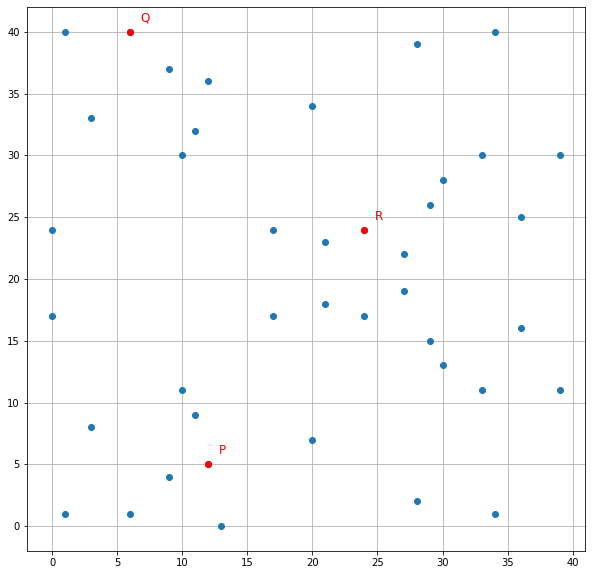
\includegraphics[width=\linewidth]{plot_corps_fini_p41.png}
\end{columns}
\end{frame}

% --- Simulation d'Attaque par force brute ---
\begin{frame}{Simulation d'Attaque : Force Brute}
\frametitle{Simulation d'Attaque : Force Brute}

Le but de l'attaque est de trouver la clé privée $d$ à partir de la clé publique $Q=d \cdot G$.

\begin{itemize}
    \item On connaît : Clé publique $Q$, paramètres $a, b, p$, et le point générateur $G$.
    \item On teste toutes les clés privées candidates $d_{cand} \in [1, n-1]$.
    \item On vérifie si $d_{cand} \cdot G = Q$.
\end{itemize}

\begin{columns}
    \column{0.5\textwidth}
    \begin{exampleblock}{Simulation avec $n=19792$}
        Courbe plus complexe : $p=78791, n=19792$
        \begin{itemize}
            \item Clé privée (vraie) : \textbf{11743}
        \end{itemize}
    \end{exampleblock}
    
    \column{0.5\textwidth}
    \begin{alertblock}{Brute force avec n = 19792}
	Clé privée trouvée : 11743 en 3.7 secondes
	\end{alertblock}

    \begin{alertblock}{Conclusion de la Simulation}
        L'attaque est \textbf{rapide} car le corps fini $p=78791$ est minuscule.
        \textbf{Dans la réalité}, les courbes utilisent $n \approx 2^{256}$.
    \end{alertblock}
\end{columns}
\end{frame}

% --- Sensibilité de l'ECDSA et Conclusion ---
\begin{frame}{Sécurité et Implémentation}
\frametitle{Le danger des implémentations manuelles}

\begin{block}{Le Danger du Nonce $r$}
La signature ECDSA dépend du nonce $r$ (nombre aléatoire secret, $r \in [1, n-1]$).

\begin{itemize}
    \item \textbf{Une réutilisation, une prévisibilité, ou une fuite partielle de $r$} permet à un attaquant de \textbf{calculer la clé privée $d$ en quelques secondes}.
    \item L'implémentation "à la main" est à proscrire : \textbf{elle est uniquement à but pédagogique}.
\end{itemize}
\end{block}

\begin{alertblock}{La Seule Approche Sécurisée}
\textbf{Utiliser des librairies cryptographiques officielles et auditées} (comme OpenSSL, Bouncy Castle, modules Python/Go).
\begin{itemize}
    \item Elles intègrent des contre-mesures strictes (attaques par canal auxiliaire).
    \item Elles garantissent la qualité cryptographique du nonce $r$.
\end{itemize}
\end{alertblock}
\end{frame}

\begin{frame}{Les Courbes Elliptiques dans la Vie Réelle}
\frametitle{Principales Courbes Utilisées pour la Signature et l'Échange de Clés}

\centering
\begin{tabular}{|l|c|c|l|}
\hline
\textbf{Nom Courbe} & \textbf{Type} & \textbf{Taille (bits)} & \textbf{Usage Principal} \\
\hline
\textbf{NIST P-256} & Courbe Prime (\texttt{secp256r1}) & 256 & Standard Web (TLS/SSL,\\ &&&Certificats) \\
\hline
\textbf{secp256k1} & Courbe Koblitz & 256 & Cryptomonnaies\\ &&&(Bitcoin, Ethereum) \\
\hline
\textbf{Ed25519} & Courbe Edwards Torsadée & 255 & Protocoles Modernes \\&&&(SSH, Signal) \\
\hline
\end{tabular}

\vspace{0.2cm}

\begin{alertblock}{Le Choix Clé : Efficacité}
    Toutes ces courbes offrent un niveau de sécurité équivalent à une clé RSA de 3072 bits, mais avec des clés 12 fois plus petites et des calculs plus rapides.
\end{alertblock}

\vspace{0.2cm}

\begin{exampleblock}{Ressource Complémentaire}
    Pour obtenir plus de détails sur les paramètres de ces courbes :
    
    \centering
    \textbf{Normes des Courbes Elliptiques : } \url{https://std.neuromancer.sk/}
\end{exampleblock}
\end{frame}
